\section{The \Sys Compiler}
\label{sec:compiler}
This section presents the \sys compiler, which takes a computation graph and an associated inference configuration as input and generates an optimized \graph specialized for both the target configuration and underlying GPU architecture. \Cref{fig:compiler_workflow} outlines the end-to-end compilation workflow.

\begin{figure*}
    \centering
    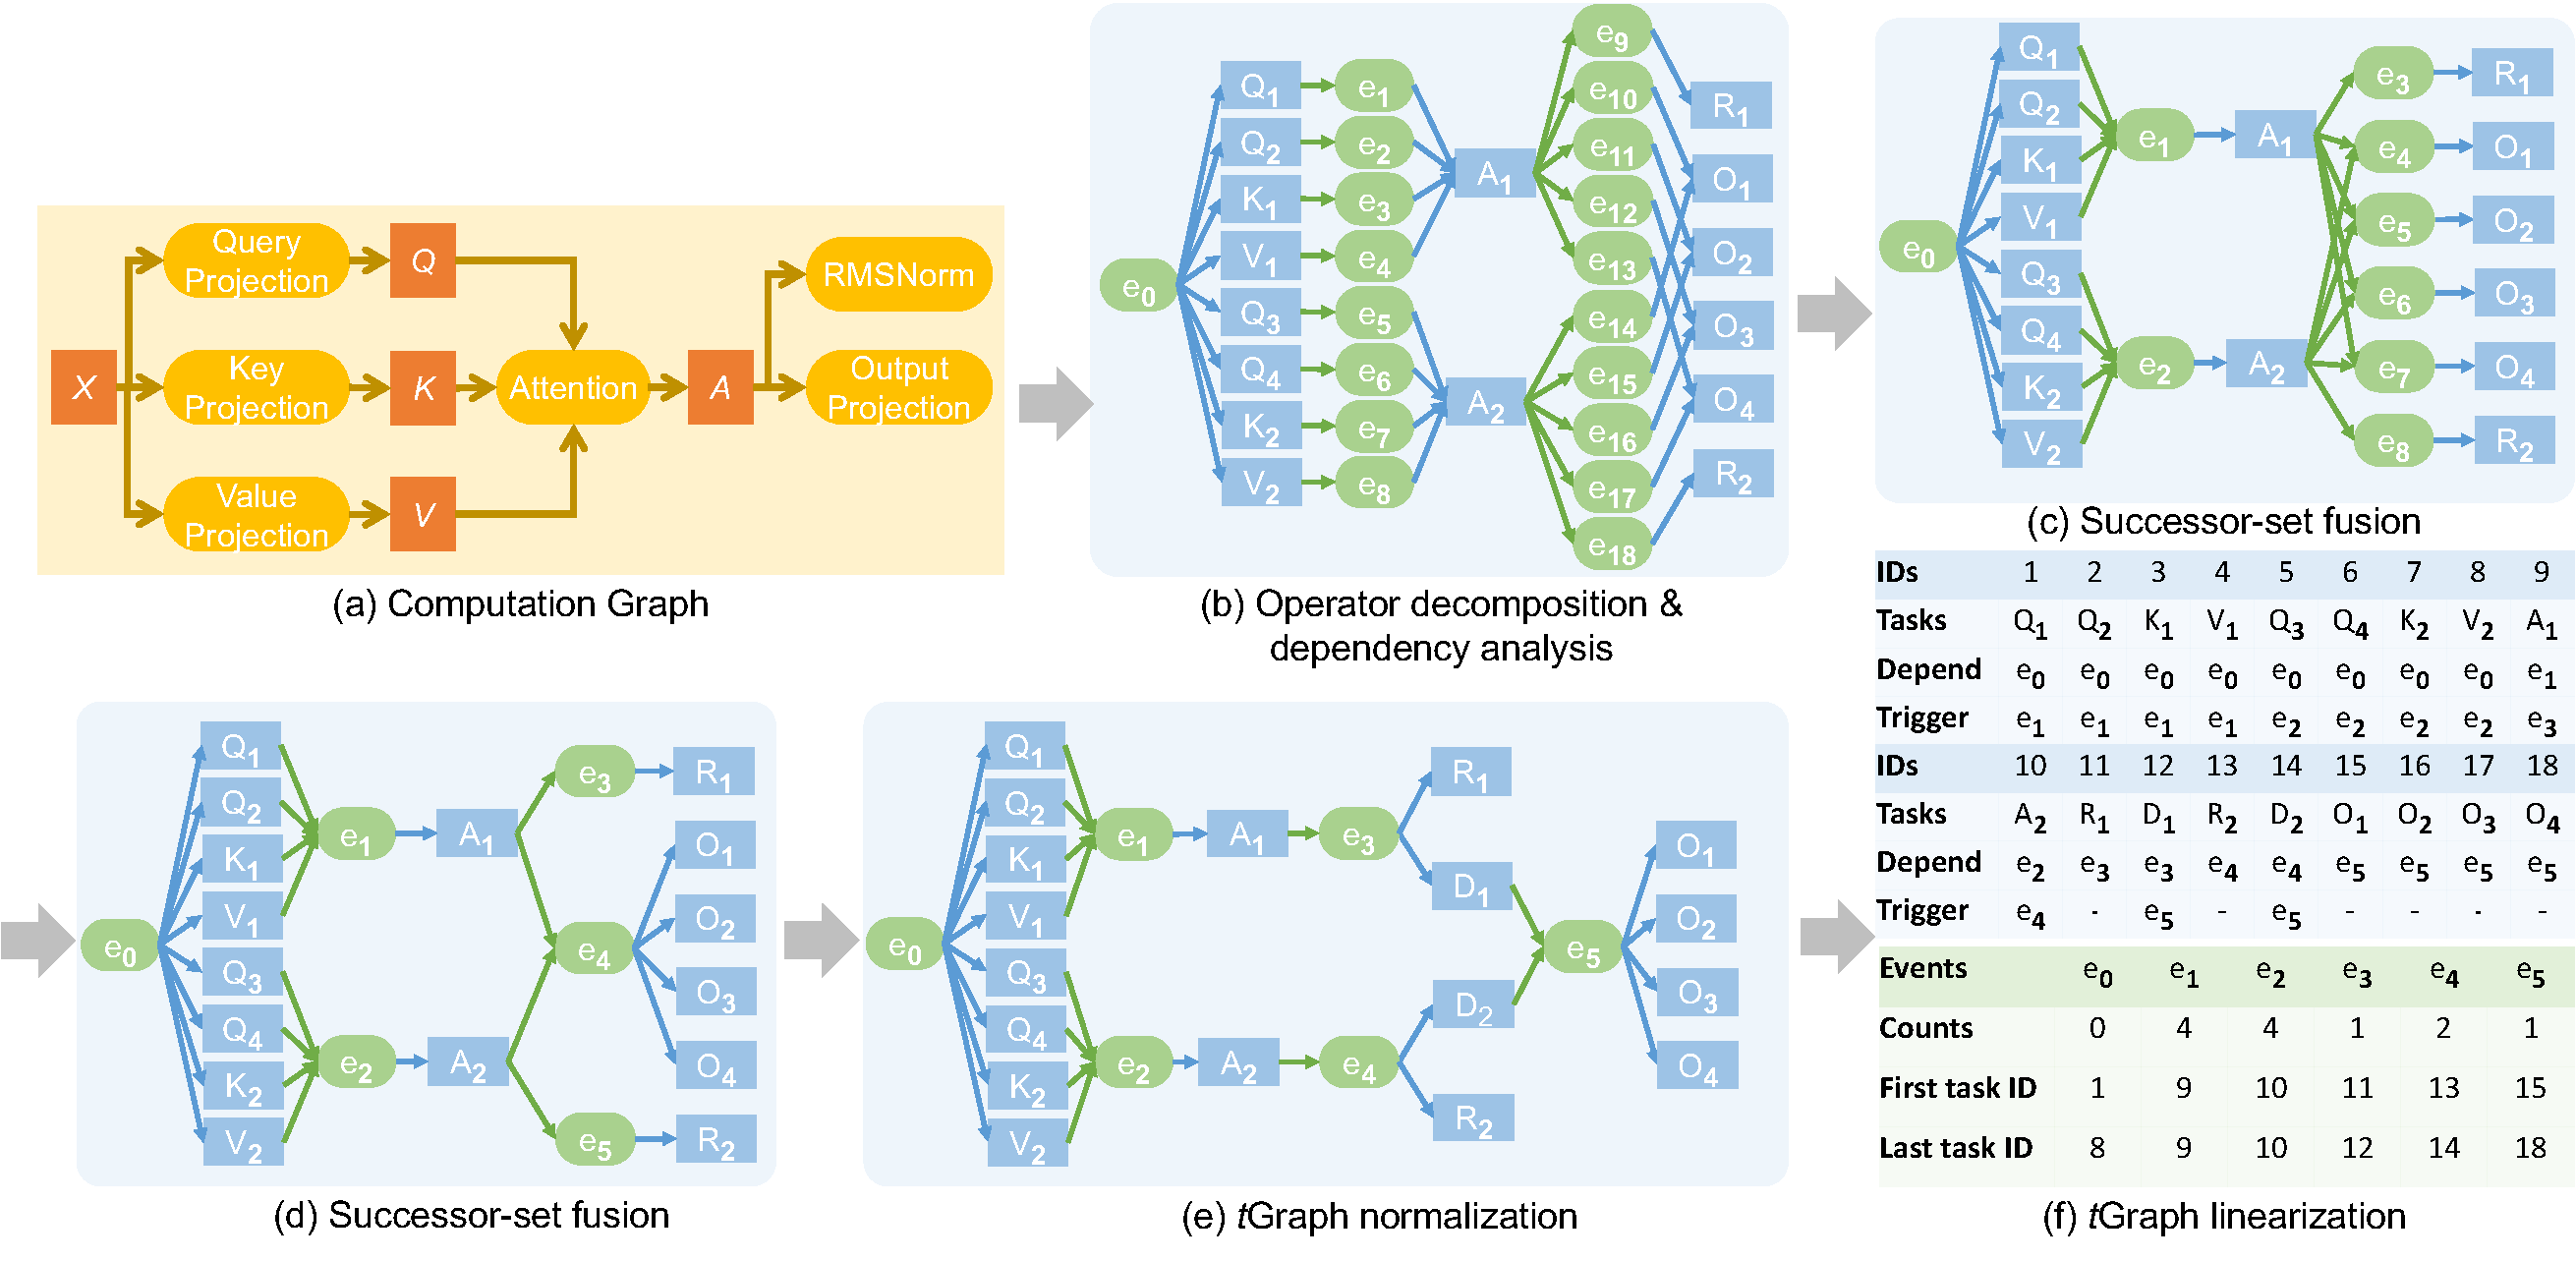
\includegraphics[scale=0.39]{figs/compiler_workflow_v3.pdf}
    \vspace{\captionvspace}
    \caption{The \sys compiler workflow. In (b), $Q$, $K$, $V$, $A$, $O$, and $R$ denote the set of tasks produced by decomposing the query projection, key projection, value projection, attention, output projection, and RMSNorm operators, respectively. $D_1$ and $D_2$ in (e) are dummy tasks inserted during \graph normalization to guarantee that each task has exactly one triggering event. Finally, (f) shows how \Sys linearizes the \graph and stores the resulting structure in GPU memory, where both tasks and events follow a uniform, canonical representation.}
    \vspace{\captionvspace}
    \label{fig:compiler_workflow}
\end{figure*}

\subsection{\graph Generation}
\paragraph{Operator decomposition.}
The \sys compiler decomposes each operator of the input computation graph into a set of tasks by {\em partitioning} the operator’s output tensors such that all tasks compute {\em disjoint} subsets of the output and can therefore execute in parallel across SMs. Most tensor algebra operators can be partitioned across multiple output dimensions; for example, the output tensor of a matrix multiplication can be tiled along both the row and column dimensions to expose parallelization opportunities.

The performance of a partitioning strategy depends on both the problem shape and the target GPU architecture. To discover an effective strategy, \sys selects a partitioning strategy that minimizes data loading from device memory to shared memory, since accessing device memory is significantly more expensive than accessing shared memory or performing computation on CUDA cores or tensor cores. By default, \sys generates a number of tasks proportional to the number of SMs to promote load balance across SMs during execution. \Sys also provides an interface for users to easily specify custom partitioning strategy by setting the desired parallelization degree along each output dimension.

\paragraph{Dependency analysis.} \Sys uses {\em events} to capture dependencies between tasks. For any two operators that share a tensor, \sys enumerates all pairs of tasks from the two operators and introduces an event $e$ for a task pair $(t_1, t_2)$ if and only if the output region produced by task $t_1$ overlaps with the input region consumed by task $t_2$. The event serves as a synchronization point indicating that $t_2$ cannot begin execution until $t_1$ has completed producing the required data. Accordingly, \sys inserts two edges $(t_1, e)$ and $(e, t_2)$ into the resulting \graph. This fine-grained dependency analysis preserves all producer-consumer dependencies while exposing maximal parallelism across independent tasks.

\paragraph{Event fusion.} \Sys applies two complementary forms of event fusion---{\em successor-set} and {\em predecessor-set} fusion---to eliminate redundant synchronization points and simplify the constructed \graph. 
For an event $e$, we define two functions: $\er{InTasks}(e)$, the set of tasks that trigger $e$, and $\er{OutTasks}(e)$, the set of tasks that depend on $e$.
These functions allow us to characterize when multiple events exhibit identical dependency structure and can therefore be fused.

First, {\em successor-set fusion} merges events that serve as prerequisites for the same set of consumer tasks. Because these tasks cannot begin execution until all such events are activated, representing them separately provides no additional scheduling flexibility.

\begin{definition}[Successor-set fusion]
For any two events $e_1$ and $e_2$ of a \graph, successor-set fusion applies if and only if $\er{OutTasks}(e_1) = \er{OutTasks}(e_2)$. \Sys removes events $e_1$ and $e_2$ from $\cal{T}$ and introduces a fused event $e'$ with $\er{InTasks}(e') = \er{InTasks}(e_1) \cup \er{InTasks}(e_2)$ and $\er{OutTasks}(e') = \er{OutTasks}(e_1)$.
\end{definition}

As an example, successor-set event fusion fuses events $e_10$ and $e_{14}$ in \Cref{fig:compiler_workflow}(b) into a new event (i.e., $e_4$ in \Cref{fig:compiler_workflow}(c)) since they are both prerequisites for task $O_1$.

Second, {\em predecessor-set fusion} merges events that depend on an identical set of producer tasks. Because such events are triggered simultaneously, maintaining them as separate synchronization nodes introduces unnecessary graph complexity.

\begin{definition}[Predecessor-set fusion]
For any two events $e_1$ and $e_2$ in a \graph $\cal{T}$, predecessor-set fusion applies if and only if $\er{InTasks}(e_1) = \er{InTasks}(e_2)$. \Sys removes events $e_1$ and $e_2$ from $\cal{T}$ and introduces a fused event $e'$ with $\er{InTasks}(e') = \er{InTasks}(e_1)$ and $\er{OutTasks}(e') = \er{OutTasks}(e_1) \cup \er{OutTasks}(e_2)$.
\end{definition}

As an example, predecessor-set fusion fuses events $e_4$, $e_{5}$, $e_6$, and $e_7$ in \Cref{fig:compiler_workflow}(c) into a single new event ($e_4$ in the new \graph) as all these events depend on tasks $A_1$ and $A_2$. 

A core challenge \Sys must address is representing dependencies between tasks and events. Because \Sys executes tasks and updates events in parallel across SMs, the runtime requires a {\em uniform} and {\em cheap} representation that avoids costly indirect indexing. Two challenges arise. First, a task may depend on and trigger an arbitrary number of events. A straightforward approach to representing tasks is reserving space for the maximum number of dependent and triggering events per task. However, this approach leads to significant memory overhead. Second, after event fusion, an event may trigger an arbitrary number of tasks. Representing these outgoing edges by allocating space for the maximum fan-out per event is also expensive.
\Sys introduces two techniques to address these challenges: \graph normalization and linearization.

\begin{figure}
    \centering
    \subfloat[A transformation reducing\\fan-out of a task to one.]{
    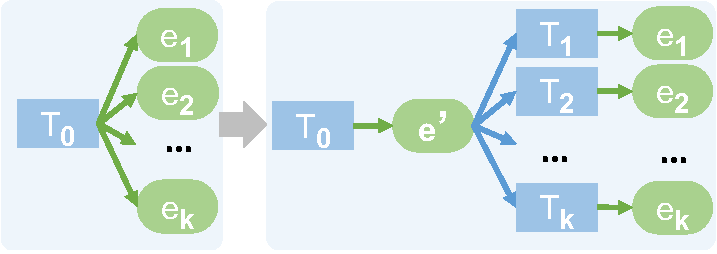
\includegraphics[scale=0.33]{figs/rewrite_1.pdf}
    \label{fig:rewrite_1}
    }
    \subfloat[A transformation reducing\\fan-in of a task to one.]{
    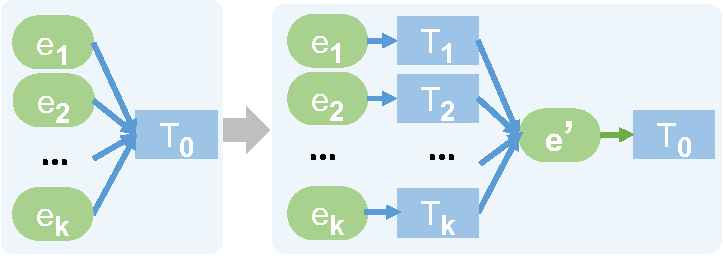
\includegraphics[scale=0.33]{figs/rewrite_2.pdf}
    \label{fig:rewrite_2}
    }
    \vspace{\captionvspace}
    \caption{\Sys performs graph transformations to normalize an arbitrary \graph, ensuring that every task has at most one dependent event and one triggering event.}
    \vspace{\captionvspace}
    \label{fig:rewrites}
\end{figure}

\paragraph{\graph normalization.} \Sys addresses the first challenge through \graph normalization, which transforms an input \graph into functionally a equivalent form where each task has at most {\em one} dependent event and {\em one} triggering event. \graph normalization is achieved by performing two types of transformations to reduce the maximum fan-in and fan-out of each task to at most one. First, when a task $T_0$  triggers multiple events $e_1,...,e_k$ in an input \graph, \sys transforms the \graph by introducing a new event $e'$ and $k$ empty new tasks $T_1,...,T_k$, each performing no computation and depending on $e'$. After this transformation, task $t_0$ triggers only $e'$, and each newly introduced task $T_i$ triggers exactly one of the original event $e_i$, as shown in \Cref{fig:rewrite_1}. 
This transformation ensures that every task has exactly one {\em triggering} event. \Cref{fig:compiler_workflow}(e) shows how \sys applies this transformation to reduce the number of triggering events for $A_1$ and $A_2$ to one.

Second, when a task $T_0$ depends on multiple events $e_1, ..., e_k$ in an input \graph, \sys transforms the \graph by introducing a new event $e'$ and $k$ empty new tasks $T_1,...,T_k$, each performing no computation and triggering $e'$. After this transformation, task $T_0$ and each newly introduced task $T_i$ depends on exactly one event, as shown in \Cref{fig:rewrite_2}.

\graph normalization introduces an overhead of adding additional tasks and events to normalize a \graph when it has tasks with multiple fan-in and fan-out events. This generally only happens when the original computation graph has operators that can execute in parallel. For example, tasks $A_1$ and $A_2$ in \Cref{fig:compiler_workflow}(d) have two fan-out events because RMSNorm and output projection operators in the original computation graph both depend on attention and can run in parallel. In practice, we observe negligible normalization overhead (i.e., always less than 1\% in our evaluation) as real-world models are ``deep'' (many sequential operators) instead of ``wide'' (many parallelizable operators).

\begin{algorithm}
\caption{\sys's \graph linearization algorithm. It is guaranteed that each task is enqueued into $T$ once and that each event is enqueued into $E$ once. Lines \ref{line:start}-\ref{line:end} ensure that all tasks depending on an event are consecutive in $T$.}
\label{algo:linearization}
\footnotesize
\begin{algorithmic}[1]
\Require{A normalized \graph $\mathcal{G}$}
\Ensure{A list of tasks $T$ such that for each event $e \in \mathcal{G}$, the set of tasks $e$ launches are consecutive in $T$.}
\State $T \gets \varnothing$
\State $E \gets \{e \in \m{G}| e.{\rm counts}=0\}$ \Comment{Enqueue all events with no dependent tasks}
\While{$E$ is not empty}
\State $e \gets E.{\rm dequeue()}$
\ForAll{task $t \in \m{G}$}\label{line:start}
\If{$t.{\rm dependent\_event} = e$}
\State $T.{\rm enqueue}(t)$\label{line:end}
\State $e' \gets t.{\rm trigger\_event}$
\If{all tasks triggering $e'$ are in $T$}
\State $E.{\rm enqueue}(e')$
\EndIf
\EndIf
\EndFor
\EndWhile
\State
\State \Return $T$
\end{algorithmic}
\end{algorithm}

\paragraph{\graph linearization.} \graph normalization alone cannot address the second challenge: after fusion, an event may still need to trigger a large number of tasks (e.g., event $e_5$ in \Cref{fig:compiler_workflow}(e) triggers four tasks), requiring additional storage to record their indices. \sys resolves this issue using a {\em breadth-first search} (BFS)-based algorithm (see \Cref{algo:linearization}) to linearize a \graph. The linearization ensures that all tasks triggered by the same event are assigned contiguous indices in the final task ordering. As a result, the fan-out of an event can be encoded compactly using only the first and last task indices, eliminating the need to store an explicit list of dependent tasks while preserving all dependency semantics. 

\Cref{fig:compiler_workflow}(f) illustrates how \sys stores the linearized \graph in GPU device memory. For each task, \sys records only the indices of its dependent and triggering events. For each event, \sys stores the number of triggers required for the event to be activated; once activated, the runtime launches all tasks whose indices fall within the event’s first and last task indices.

\subsection{Task Implementation Generation}
In addition to constructing a \graph, \sys also needs to generate a device function for each task to be executed on a GPU SM. \sys leverages prior work and employs a {\em compiler superoptimization} approach to automatically generating a high-performance implementation for each task.
Specifically, \sys performs superoptimization at the thread block level instead of the kernel level. Each compute task is associated with a reference PyTorch implementation, and \sys leverages the Mirage superoptimizer~\cite{wu2025mirage} to automatically search for an optimal thread block graph, which is sent to the Mirage compiler for generating a CUDA implementation. The CUDA implementation includes all intra-SM optimizations such as software pipelining, register reusing, and layout optimizations to minimize bank conflicts.


